In order to connect the continuous classical models of light with this work discrete numerical designs we start by comparing the numerical results for aberrations in the normalized Luneburg lens with analytic solutions. \footnote{Analytically, Luneburg conjecture yields zero aberration}. Thus, aberrations in the super-lens in the order of the aberrations in the Luneburg lens are acceptable and reported as free aberrations. \\

\subsection{Relevant Design parameters and relations}
In order to make a proper optimization of the super-lens, its necessary to understand the relations between the system parameters. Firstly, note that the  focal distance of the first array of lenses determines the spread of the parameter $\beta_n$. In addition, larger values for this spread allow for bigger radius on the third layer $R_3^n$  which leads to smaller values of aberrations (Err) as a result of,
\begin{equation}
    Err \propto \frac{f}{R}
\end{equation}

There exists another relation between the maximum height of incidence (H) in the third array and the radius of the second array of lenses. The smaller the radius, the lower the rays leading to smaller aberrations of the third array and overall system. This relation can also be understood with optical magnification. Thus, it is important to respect $R_2^n < R_3^n$.
\begin{equation}
    Err \propto H_f \propto \frac{f}{R}
\end{equation}

Finally, the relation to the spread on $\beta_n$  and the focal distance of the super-lens dictates to minimize the spacing between the second and third layer without sacrificing too much height (H). Thus, for the last layer, it is also convenient to set a limit on the ratio

\begin{equation}
    Err  \propto \frac{H_f}{R} \propto  \frac{1}{ft-f_1+f_3}.
    \label{eq:errproptoh}
\end{equation}


\subsection{Individual lens Optimization}
The Luneburg conjecture leads to the conclusion that each lens can have zero aberration for a finite focal length. Furthermore, the Gutman lens, whose refractive index profile is given by
\begin{equation}
    n(r) = \sqrt{\frac{R^2+f^2-r^2}{f^2}},
\end{equation}
has the property of focusing rays outside the lens but with spherical aberration. To overcome such aberrations it is possible to introduce correction factors to the distribution that help minimize such aberrations. This has benn done previusly by Zhao. et al \cite{zhao} but the results they reported where false and presented aberrations in our numerical simulations. Thus, in order to make a proper optimization we introduced the following distribution with 3 degrees of freedom: $\alpha,\beta,R$ and
\begin{equation}
    n(r) = [\frac{R^2+f^2-\alpha r^2}{f^2}]^\beta.
\end{equation}

Introducing the factor $\beta$ allows for control over the aberrations of rays outside the paraxial height. This is important because the objective is to capture a wide FOV. In particular, the optimization of beta becomes relevant in the first layer because $H_f=R_1^n$ and the relation with the aberration given by \ref{eq:errproptoh}. For the first lens array we obtained the following results. 
\begin{center}
    \begin{table}[H]
    \resizebox{\columnwidth}{!}{ % Scale to column width
    \begin{tabular}{|c|c|c|c|c|c|}
    \hline
    \textbf{R} & \textbf{$\alpha$} & \textbf{$\beta$} & \textbf{$f$} & \textbf{$z_{ave}$} & \textbf{Err} \\ \hline
    $R_1^n=1$    & 0.86              & 0.5285              & 1.2315          & 1.3              & 9.3e-4        \\ \hline
    \end{tabular}
    } % End resizebox
    \end{table}
\end{center}


Note that, our numerical optimizations have limits and strongly depend on the computing power and discretization available. Its worth mentioning that the latter results are obtained with a step size L = 0.00005 \footnote{In a unit radius, the center ray travels 40,000 steps. }. In this regime, the numerical aberrations for the Luneburg lens lie on the order of e-4, meaning the super-lens presented has to present aberrations of this same order.\\

The focal distance of the system is set to $6 [r_{units}]$. This is related to the optimization the work wishes to present. To optimize the spatial dimension of the problem, its realistic to propose a $60\%$ reduction. This means that a wave front of 10 units is focused on 6 rather than 10 in the case of the lunemburg lens i.e $f_t = 6 [units]$. \\

Starting from the first layer, with the radius of the lenses unitary, the focal distance is $f_1 = z_ave1=1.3$.  In order to maximize the individual radius of the third layer $R_3^n$, a geometrical relation can be implemented so that all the space is covered while the lenses still lie on the circumference of the curve characteristic of the third layer. To do so, its necessary to fix the radius center lens. For our design we choose $R_3^0 = 0.439$ so that $R_3^1 =R_3^2 = 0.265$. One last optimization consists on finding the optimal GRIN distribution for the third layer lenses. The results obtained are the following.

\begin{center}
    \begin{table}[H]
    \resizebox{\columnwidth}{!}{ % Scale to column widt
    \begin{tabular}{|c|c|c|c|c|c|}
    \hline
    \textbf{R}         & \textbf{$\alpha$} & \textbf{$\beta$} & \textbf{$f$} & \textbf{$z_ave$} & \textbf{Err} \\ \hline
    $R_3^0=0.439$      & 0.745             & 0.5              & 1.049        & 1.7              & 0.001        \\ \hline
    $R_3^1=R_3^2=0.26$ & 0.779             & 0.5              & 0.764        & 1.7              & 0.009        \\ \hline
    \end{tabular}
    } % End resizebox
    \end{table}
\end{center}

The full ensemble of the super lens gives a total aberration of 0.03. This means that the optimization with the specific characteristics presents aberrations with three orders of magnitude greater than perfect focus. The system is presented in figure \ref{fig:superlens_v1}

\begin{figure}[H]
    \centering
    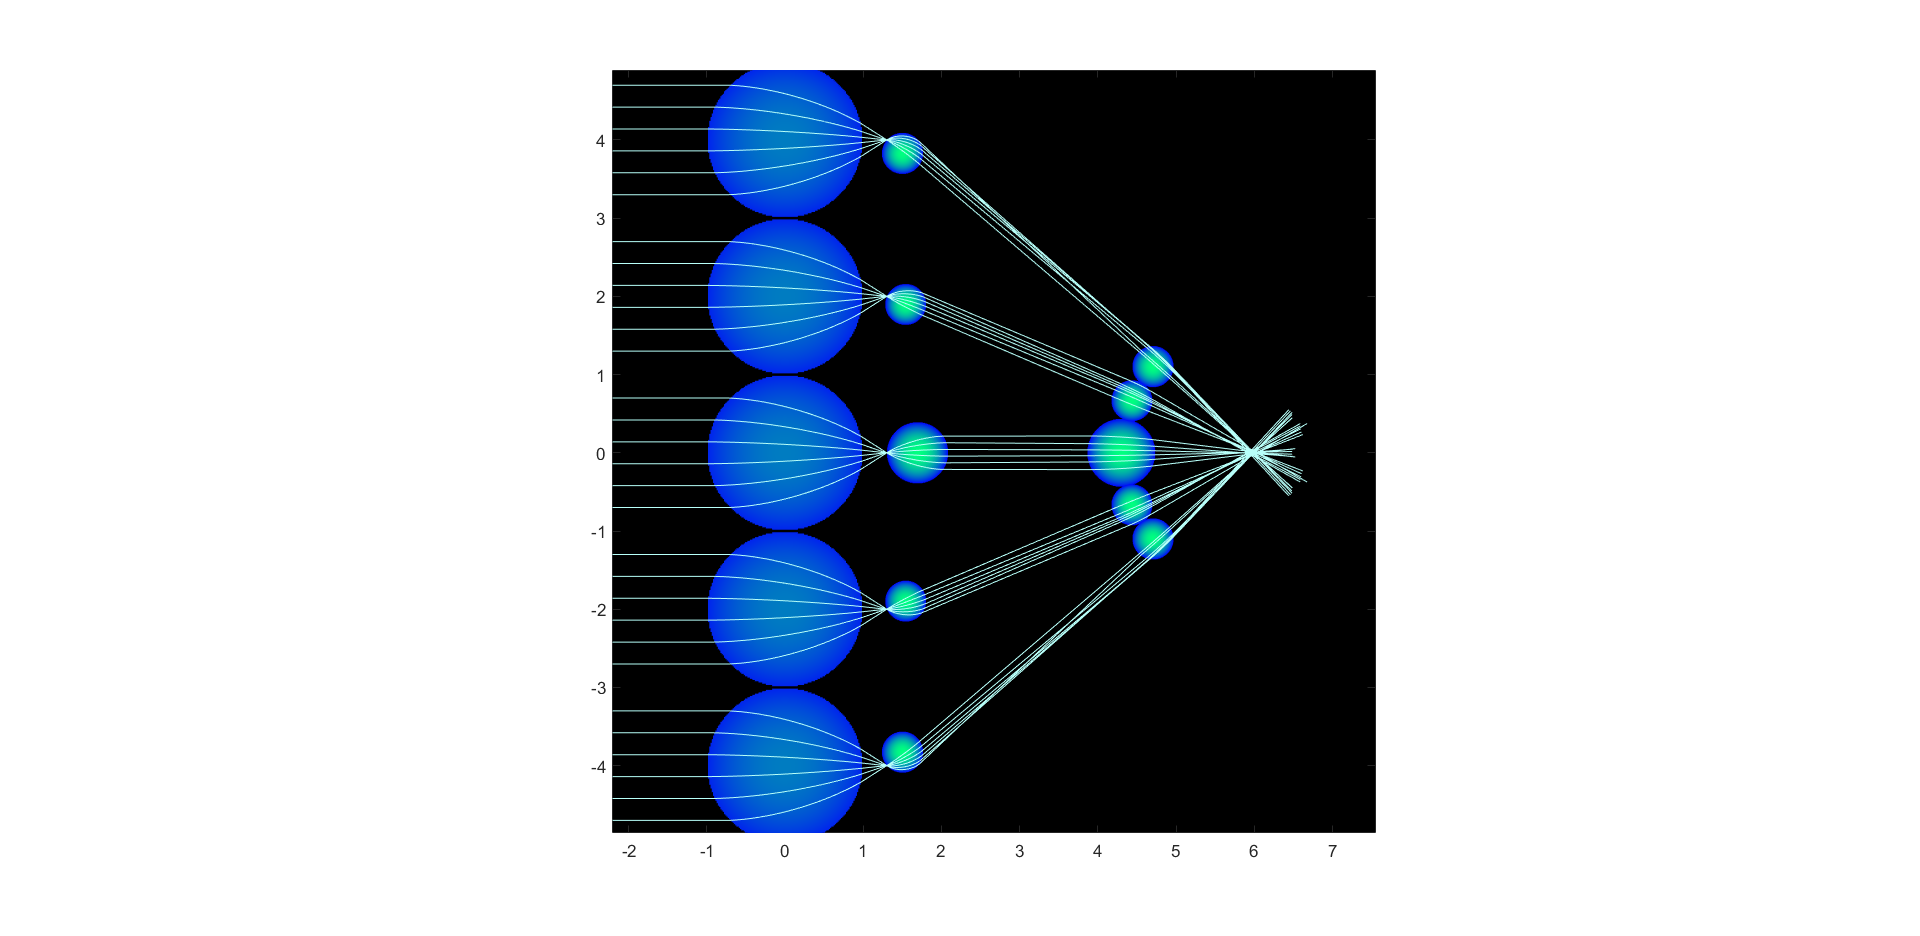
\includegraphics[scale=0.2]{Figures/MYSuperlens_final.png}
    \caption{Super-lens distribution}
    \label{fig:superlens_v1}
\end{figure}